\documentclass[12pt,a4paper]{article}
\usepackage[utf8]{inputenc}
\usepackage[german]{babel}
\usepackage[T1]{fontenc}
\usepackage{amsmath}
\usepackage{amsfonts}
\usepackage{amssymb}
\usepackage{graphicx}
\usepackage{siunitx}
\usepackage{float}
\usepackage[left=2cm,right=2cm,top=2cm,bottom=2cm]{geometry}
\usepackage{hyperref}
\author{Gerald}


\begin{document}
\sisetup{separate-uncertainty = true}
	\setlength{\parindent}{0pt} 
	\begin{center}
		{\LARGE Versuchsprotokoll}\\
		\begin{large}
			zum Fortgeschrittenenpraktikum im Bachelorstudiengang Physik\\[0.4cm]
			an der RWTH Aachen\\
			II. Physikalisches Institut A\\[5.5cm]
			\Large\textbf{\textsl{Röntgenspektroskopie (T06)}}\\[5.5cm]
			\normalsize\textit{vorgelegt\\von}\\[0.4cm]
			\large{Moritz Berger (355244)\\Gerald Kolter (355005)}\\\textbf{Gruppe 30}\\[2cm]
			\large \textbf{Wintersemester 2017/18}
		\end{large}
	\end{center}
	\newpage
	
	\tableofcontents
	\newpage
	
\section{Hintergund}
Wenn man Materialien mit hochenergetischen Teilchen bestrahlt, so wechelwirken diese folgendermaßen mit den darin enthaltenden Atomen\footnote{Quelle:}:
\begin{enumerate}
\item Bei der Bewegung durch das Material werden die Teilchen abgebremst. Die dabei freiwerdende Energie äußert sich als ein kontinuirliches elektromagnetisches Spektrum, das Bremsstrahlung genannt wird. Die Intensität dieser Strahlung nimmt mit der Masse der abgebremsten Teilchen ab.
\item Die Teilchen geben ihre Energie an ein Elekron im Atom ab, was infolgedessen ionisiert wird. Dadruch wird eine Elektronposition frei und ein höherenergetisches Elektron im Atom kann auf diese Position fallen, wobei ein Röntgenquant abgestrahlt wird. Diesem Übergang kann eine diskrete Energie zugeordent werden. In der Realität äußert er sich wegen Energieunsicherheiten als Gau
\end{enumerate}
Der zweite Effekt hängt direkt von dem Atomaufbau ab, wodurch sich das dadurch ausgestrahlte Spektrum je nach Element unterscheidet. Dadurch kann man die Zusammensetzung eines Materials untersuchen, was in diesem Versuch ausgenutzt wird.
In diesem Versuch wird sowohl ein $\alpha$-Strahler, als auch eine Röntgenquelle als Quelle der hochenergetischen Teilchen benutzt.\\
Ziel ist es, beide Aufbauten mithilfe von mehreren Proben bekannter Zusammensetzung zu kalibrieren, um dann eine Reihe von unbekannten Proben mithilfe ihrer Röntgenpeaks zu untersuchen.
\section{Aufbau}
\subsubsection{$\alpha$-Quelle}
Der erste Aufbau besteht einem X-123 Spektrometer, welches aus einem Halbleiterdetekor der Kennung XR100CR und einem digitalen Pulsprozessor DP5 besteht, der die vom Detektor regristrierten Signale verstärkt und digitalisiert. Der Detektor kann maximal Energien von c.a \SI{60}{keV} aufnehmen, da Teilchen mit größerer Energie den Detektor durchfliegen.\\
Diese Signale werden an einen PC weitergeleitet, wo sie mit dem Programm und der Software ADMCA\footnote{\url{http://amptek.com/products/dpp-mca-display-acquisition-software/}} mithilfe eines Multi-Channel-Analyzers (MCA) nach ihrer Energie auf 496 Kanäle aufgeteilt werden.\\
Zur Kalibration dieser Channels gegen die Energie wird eine variable Röntgenstrahlquelle der Kennung 0317LA benutzt, welche aus einer $^{241}AM$-Quelle besteht, die $\alpha$-Strahlung auf ein durch eine Drehscheibe variables Target strahlt. Diese Quelle wird direkt vor den Detektor gestellt.\\
Zur Aufnahme von unbekannten Proben wird eine $^{241}AM$-Quelle der Kennummer Z3715 benutzt, welche in eine Bleibefestigung eingelassen wird.
\subsubsection{Röntgenquelle}
Bei den Messungen mit der Röntgenquelle wird ein X-123 Spektrometer der gleichen Bauart wie oben beschrieben verwendet. Die Röntgenquelle hat die Kennnummer BJ8288.
\section{Durchführung}
\subsubsection{$\alpha$-Quelle}
Als erstes muss über eine Kalibration den Channels eine Energie zugeordent werden.\\
Die dafür benutzte variable Röntgenstrahlquelle besitzt 6 Targets aus verschiedenen Materialien: Cu, Rb, Mo, Ag, Ba und Tb.\\
Bevor die Messungen gestartet werden können, muss an dem benutzten Programm der richtige Messbereich eingestellt werden. Dies geschieht an dem Tb Spektrum, da diese Probe Röntgenstrahlung mit der größten Energie aussendet, welche außerdem knapp unterhalb der maximal messbaren Energie liegt.\\
Dazu wird in den Programmeinstellungen der Verstärkungsfaktor so eingestellt, dass die Linie mit der größten Energie möglichst weit rechts im sichtbaren Spektrum liegt.\\
Außerdem kann über den Reiter "shaping" eine "Pile-up Rejection"(PUR) und eine "Rise Time Discrimination"(RTD) zugeschaltet werden. Bei einer Schnellauswertung haben diese Einstellungen aber keinen nennenswerten Unterschied gemacht, weswegen sie für die Messungen deaktiviert wurden.\\
Alle Einstellung sind in Tabelle \ref{tab:alpha_Einstellungen} aufgelistet.\\
\\
Nun wird für jede der sechs Proben über \SI{15}{min} das Spektrum aufgenommen.\\
Danach werden für eine Edelstahlplatte und mehrere Münzen ebenfalls über \SI{15}{min} die Spektren aufgenommen.
\begin{table}
\centering
\begin{tabular}{|c|c|}
\hline 
Einstellung & Wert \\ 
\hline 
Gain(coarse) & 2.1x \\ 
\hline 
Gain(fine) & 0.95 \\ 
\hline 
RTD & aus \\ 
\hline 
PUR & aus \\ 
\hline 
Messzeit & 15 min \\ 
\hline 
\end{tabular} 
\caption{Einstellungen für die Messungen mit der $\alpha$-Quelle.}
\label{tab:alpha_Einstellungen}
\end{table}
\subsection{Röntgenquelle}

\section{Ergebnisse $\alpha$-Quelle}
\subsubsection{Kalibration}

\begin{figure}
\centering
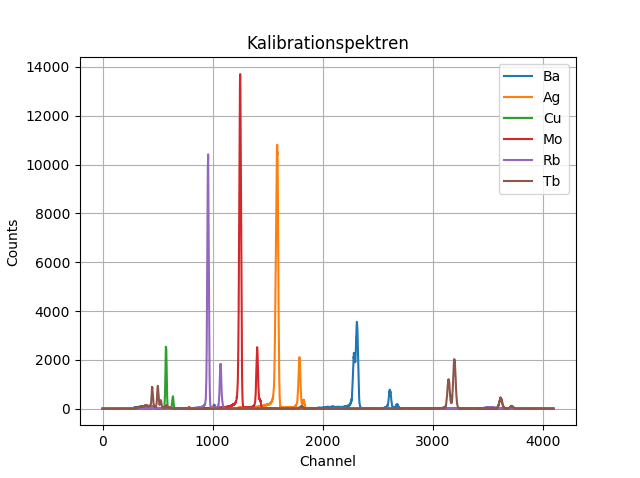
\includegraphics[scale=0.9]{Bilder/alpha/kal_alles.png}
\caption{Alle für dei Kalibration aufgenommenen Spektren.}
\label{fig:kal_alles}
\end{figure}

Die Spektren der sechs Proben sind in Abbildung \ref{fig:kal_alles} gezeigt.\\
Da das Rauschen in den Daten nicht sehr groß ist wird auf einen Frequenzcutoff verzichtet.\\
Für alle Spektren ist der $K_{\alpha}$ und der $K_{\beta}$ Peak zu sehen.
Nun wird an diese Peaks ein Gaussfit angepasst. Dies ist in Abbildung \ref{fig:kal_fits} beispielhaft gezeigt. Die restlichen Anpassungen befinden sich im Anhang.\\
Bei Peaks mit höheren Energien wird die Feinstrukturaufspaltung immer sichtbarer, bis man die Linien eindeutig trennen kann, wie in Abbildung \ref{fig:kal_fein} anhand des Barium $K_{\alpha}$-Peaks zu sehen. Da sich die beiden Linien aber immernoch überlagern, ist die sichtbare Position der Peaks leicht versetzt. Um die wahre Position bestimmen zu können, wird eine doppelte Gaußfunktion angefittet, die die Positionen beider Peaks bestimmt.\\
Die Feinstruktur tritt natürlich auch bei den niedrigenergetischen Peaks auf. Hier äußert sie sich dadurch, dass der Peak nicht exakt gaussförmig ist,sondern eine unterschiedliche Flankensteigung auf beiden Seiten hat. Dadurch verschiebt sich die Position leicht, wenn man den Anpassungsbereich vergrößert.\\
Um den Fehler auf die Position besser abschätzen zu können, wird deswegen einmal ein kleiner und einmal ein großer Bereich an die Peaks angepasst. Der Unterschied in der Peakposition wird als Fehler angenommen, solange dieser größer als der Fitfehler ist.\\
Als Peakposition wird immer die mit dem kleineren Fehler genommen, da dise den jeweiligen Peak genauer beschreibt.\\
\\
An den so bestimmten Peaks wird nun eine Energiekalibration durchgeführt. Dazu wird den Peaks eine Energie zugeordnet, die den Literaturwerten entnommen wurde, welche in Tabelle \ref{tab:alpha_lit} aufgelistet sind. Falls in einem Peak mehrere Literaturwerte liegen, so wird der Wert genommen, dessen Peak die höhere Intensität hat. Dies ist immer $K_{\alpha_1}$ und $K_{\beta_{1}}$.\\
Nun wird eine lineare Regression durchgeführt, die den Channels eine Energie zuweist. Dies ist in Abbildung \ref{fig:kal_linreg} zu sehen. Daraus ergibt sich eine Kalibrationsgrade von
\begin{equation}
E = (0.013904\pm0.000004)\cdot CH + (0.060\pm0.010)
\end{equation}
wobei die Energie in keV angegeben wird.

\begin{table}
\centering
\begin{tabular}{|c|c|c|c|c|}
\hline 
Probe & $K_{\alpha_1}$ & $K_{\alpha_2}$ & $K_{\beta_2}$ & $K_{\beta_{1/3}}$ \\ 
\hline 
Cu & $576.8\pm0.2$ & - & -& $638.5\pm0.6$\\ 
\hline 
Rb & $958.1\pm0.1$ & - & -& $1071.5\pm0.4$\\ 
\hline 
Mo & $1249.8\pm1.5$ & - & $1430.0\pm0.9$ & $1404.1\pm0.4$ \\ 
\hline 
Ag & $1588.7\pm1.0$ & - & $1825.1\pm0.2$ & $1787.5\pm0.3$ \\ 
\hline 
Ba & $2310.1\pm0.8$ & $2282.8\pm0.9$ & $2674.6\pm0.2$ & $2609.4\pm0.3$ \\ 
\hline 
Tb & $3195.4\pm0.2$ & $3152.7\pm0.1$ & $3715.4\pm0.4$ & $3616.1\pm0.4$ \\ 
\hline 
\end{tabular} 
\caption{Peakpositionen in den Channels der abgelesenen Peaks. Falls keine Feinstrukturaufspaltung ermittelt werden konnte, wurd angenommen, dass der Peak immer der mit der größeren Intensität ist.}
\label{tab:alpha_kal}
\end{table}

\begin{table}
\centering
\begin{tabular}{|c|c|c|c|c|c|}
\hline 
Probe & $K_{\alpha_1}$ & $K_{\alpha_2}$ & $K_{\beta_2}$ & $K_{\beta_{1}}$ & ($K_{\beta_{3}}$) \\ 
\hline 
Cu & 8,047.8 & 8,027.8 & - & 8,905.3 & 8,905.3\\ 
\hline 
Rb & 13,395.3 & 13,335.8  & 15,185 & 14,961.3 & 14,951.7\\ 
\hline 
Mo & 17,479.3 & 17,374.3 & 19,965.2  & 19,608.3 & 19,590.3\\ 
\hline 
Ag & 22,162.9 & 21,990.3 & 25,456.4 & 24,942.4 & 24,911.5\\ 
\hline 
Ba & 32,193.6 & 31,817.1 & 37,257 & 36,378.2 & 36,304.0\\ 
\hline 
Tb & 44,481.6 & 43,744.1 & 51,698 & 50,382 & 50,229\\ 
\hline 
\end{tabular} 
\caption[test]{Literaturwerte\footnotemark für die Peakpositionen. Alle Angaben sind in eV, wobei nach der 1000eV stelle ein Komma steht.}
\label{tab:alpha_lit}
\end{table}
\footnotetext{Quelle: \url{http://xdb.lbl.gov/Section1/Table_1-3.pdf}}

\begin{figure}
\centering
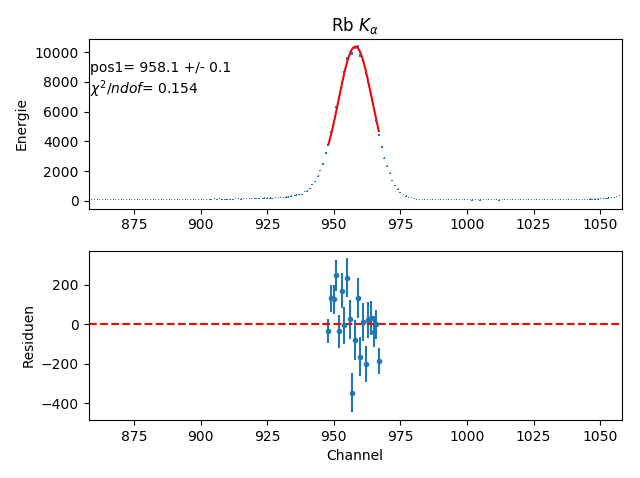
\includegraphics[scale=0.8]{Bilder/alpha/rb_alpha_1.png}
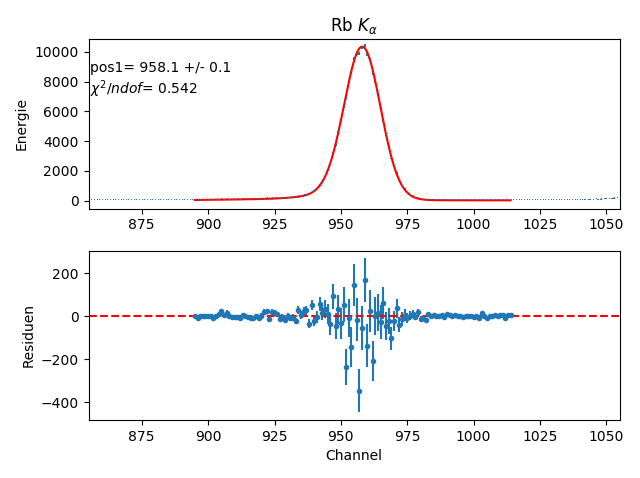
\includegraphics[scale=0.8]{Bilder/alpha/rb_alpha_2.png}
\caption{Beispiel für den Gaußfit anhand des $K_{\alpha}$ Peaks von Rubidium. In diesem Peak liegen $K_{\alpha_1}$ und $K_{\alpha_1}$ sehr eng nebeneinander, weswegen der Peak gaussförmig ist und sich die Position bei Vergrößerung kaum verändert}
\label{fig:kal_fits}
\end{figure}

\begin{figure}
\centering
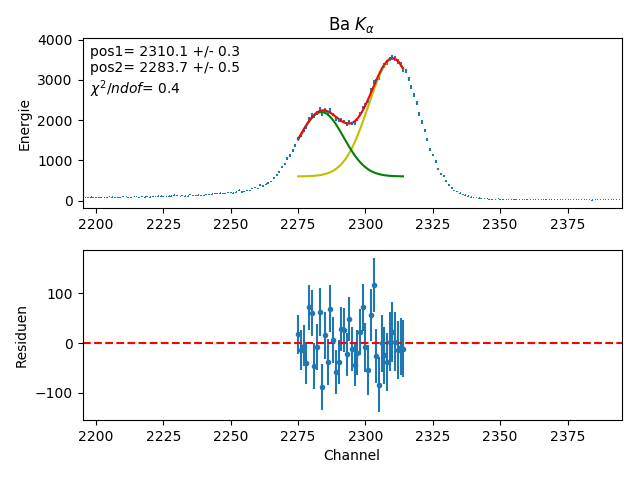
\includegraphics[scale=0.8]{Bilder/alpha/ba_alpha_1.png}
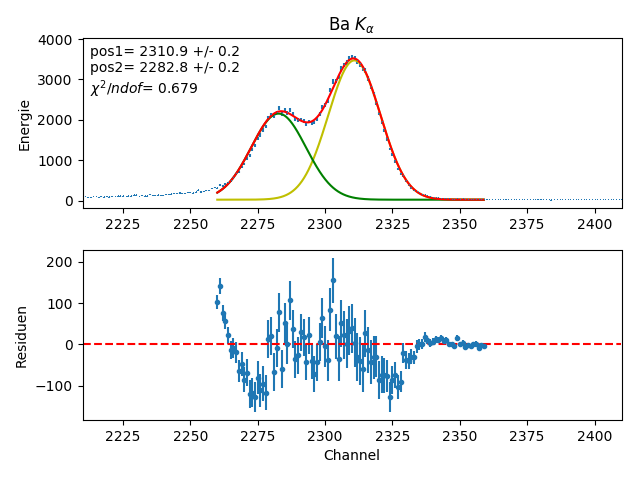
\includegraphics[scale=0.8]{Bilder/alpha/ba_alpha_2.png}
\caption{Doppelter Gaussfit (in rot) an sich überlappende Peaks. Bei der Änderung des Fitbereiches ändert sich auch die Positionder Peaks. Es sind außerdem die beiden einzelnen Peaks eingezeichnet (gelb und grün).}
\label{fig:kal_fein}
\end{figure}

\begin{figure}
\centering
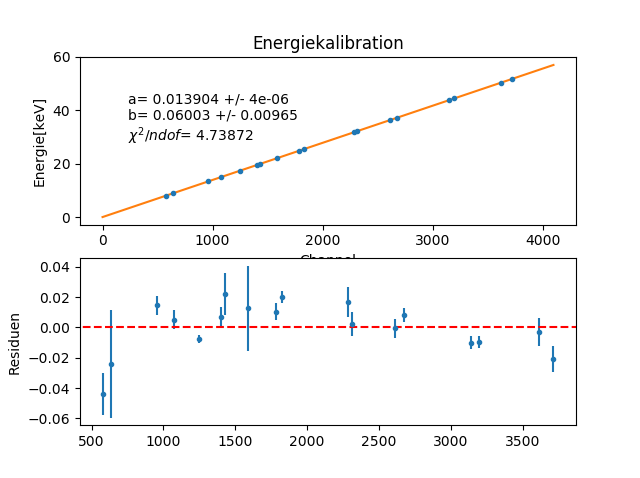
\includegraphics[scale=0.8]{Bilder/alpha/kal.png}
\caption{Lineare Regression an den Channelpositionen und der zugewiesenen Energie. Der jeweilige Fehler der Datenpunkte ist der Maximalfehler aus Fit und Fitvariation.}
\label{fig:kal_linreg}
\end{figure}

\subsubsection{Auswertung unbekannter Proben}
\subsubsection{Energieauflösung}
\section{Ergebnisse Röntgenquelle}
\subsubsection{Kalibration}
\subsubsection{Auswertung unbekannter Proben}
\subsubsection{Energieauflösung}

\section{Fazit}
\section{Anhang}
\subsection{Kalibration $\alpha$-Quelle}
\begin{figure}[H]
\centering
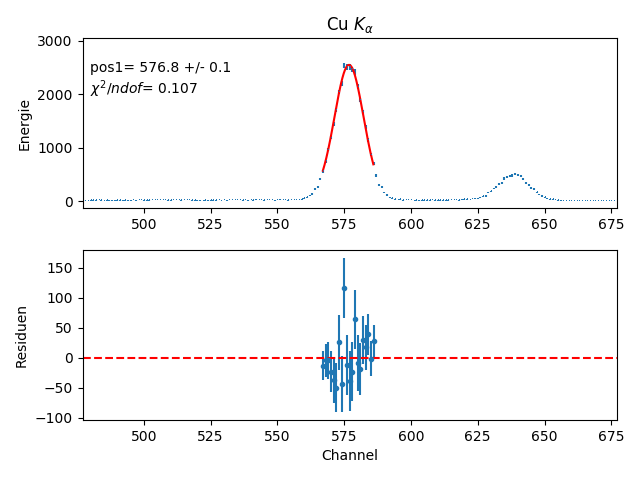
\includegraphics[scale=0.8]{Bilder/alpha/cu_alpha_1.png}
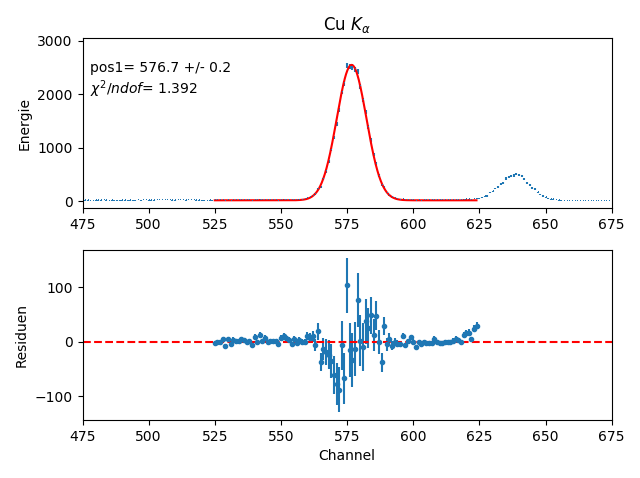
\includegraphics[scale=0.8]{Bilder/alpha/cu_alpha_2.png}
\caption{Alle für dei Kalibration aufgenommenen Spektren.}
\label{fig:kal_alles}
\end{figure}
\begin{figure}[H]
\centering
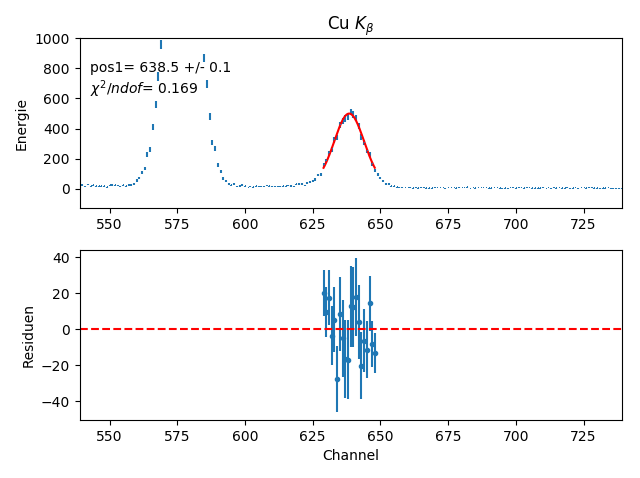
\includegraphics[scale=0.8]{Bilder/alpha/cu_beta_1.png}
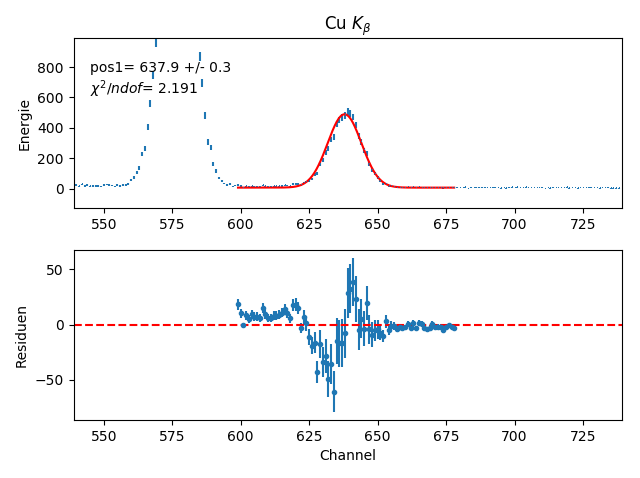
\includegraphics[scale=0.8]{Bilder/alpha/cu_beta_2.png}
\caption{Alle für dei Kalibration aufgenommenen Spektren.}
\label{fig:kal_alles}
\end{figure}

\begin{figure}[H]
\centering
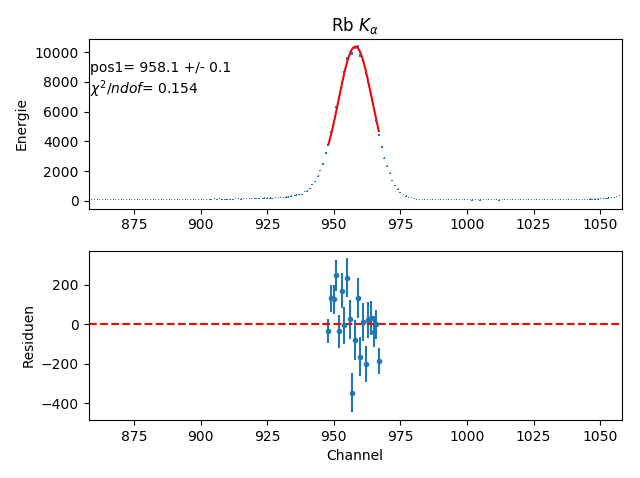
\includegraphics[scale=0.8]{Bilder/alpha/rb_alpha_1.png}
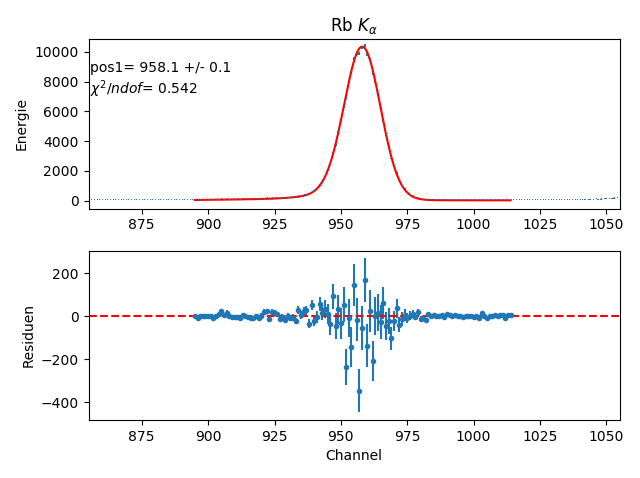
\includegraphics[scale=0.8]{Bilder/alpha/rb_alpha_2.png}
\caption{Alle für dei Kalibration aufgenommenen Spektren.}
\label{fig:kal_alles}
\end{figure}
\begin{figure}[H]
\centering
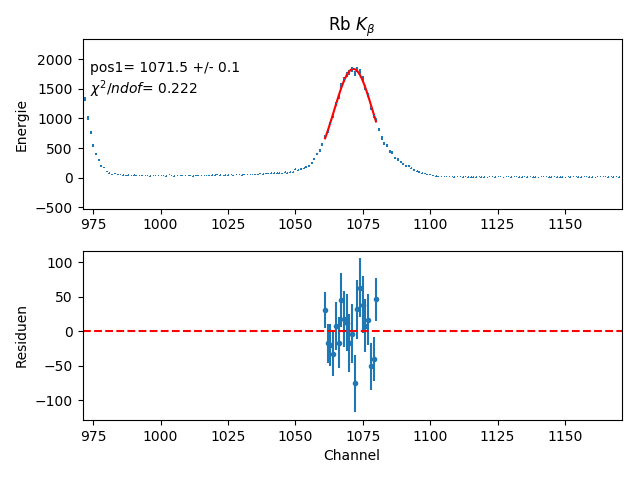
\includegraphics[scale=0.8]{Bilder/alpha/rb_beta_1.png}
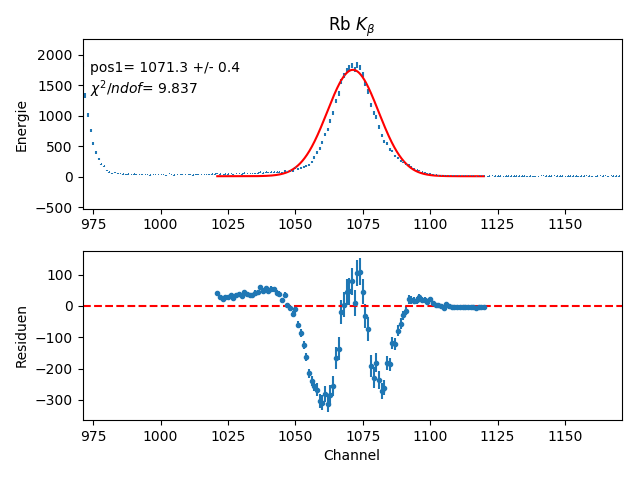
\includegraphics[scale=0.8]{Bilder/alpha/rb_beta_2.png}
\caption{Alle für dei Kalibration aufgenommenen Spektren.}
\label{fig:kal_alles}
\end{figure}

\begin{figure}[H]
\centering
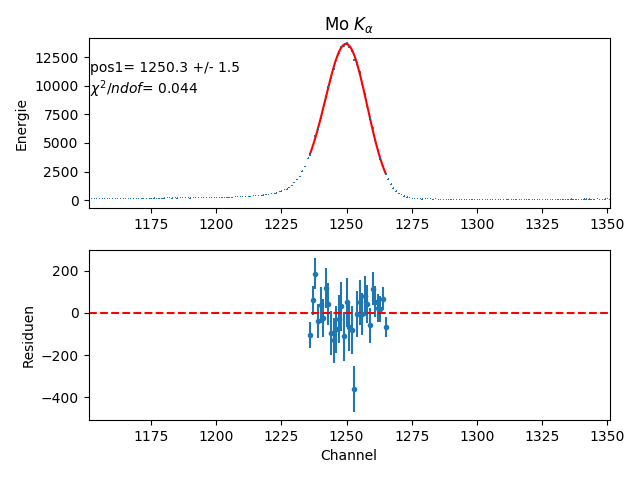
\includegraphics[scale=0.8]{Bilder/alpha/mo_alpha_1.png}
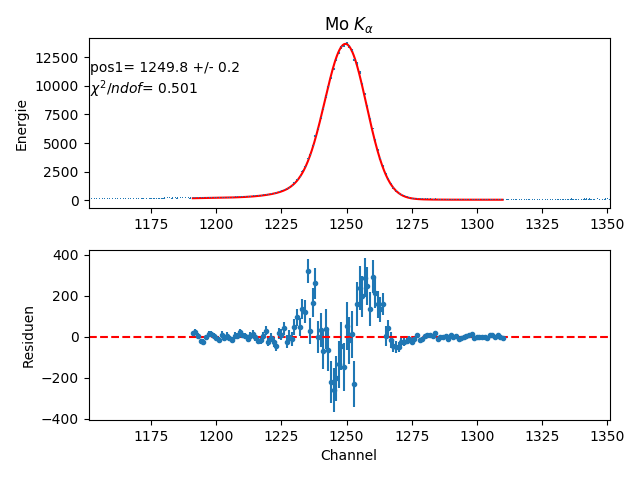
\includegraphics[scale=0.8]{Bilder/alpha/mo_alpha_2.png}
\caption{Alle für dei Kalibration aufgenommenen Spektren.}
\label{fig:kal_alles}
\end{figure}
\begin{figure}[H]
\centering
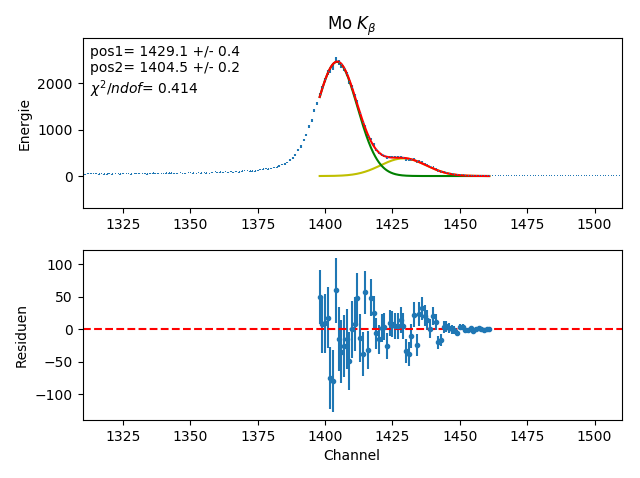
\includegraphics[scale=0.8]{Bilder/alpha/mo_beta_1.png}
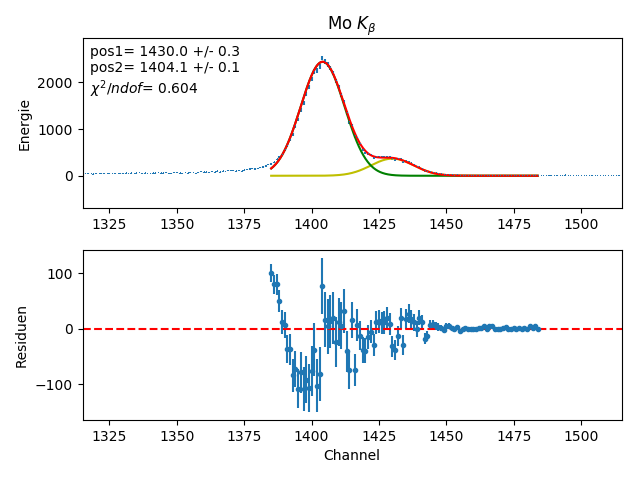
\includegraphics[scale=0.8]{Bilder/alpha/mo_beta_2.png}
\caption{Alle für dei Kalibration aufgenommenen Spektren.}
\label{fig:kal_alles}
\end{figure}

\begin{figure}[H]
\centering
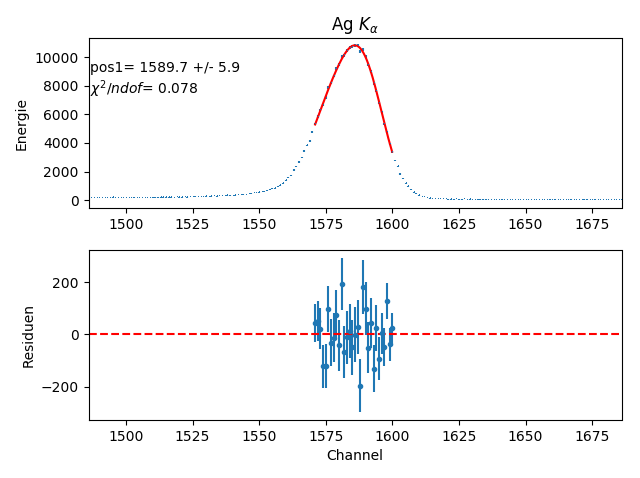
\includegraphics[scale=0.8]{Bilder/alpha/ag_alpha_1.png}
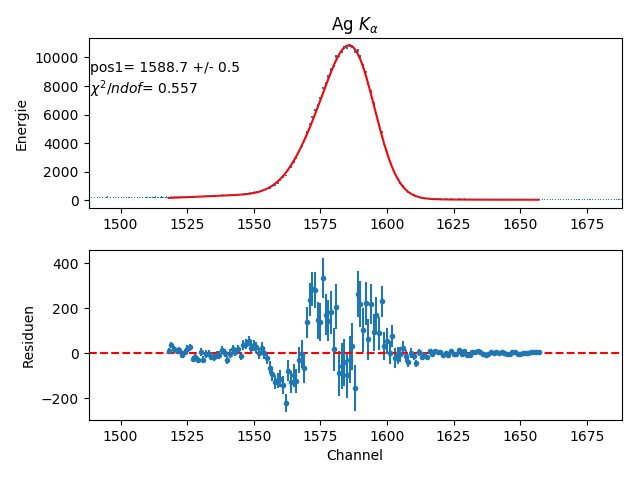
\includegraphics[scale=0.8]{Bilder/alpha/ag_alpha_2.png}
\caption{Alle für dei Kalibration aufgenommenen Spektren.}
\label{fig:kal_alles}
\end{figure}
\begin{figure}[H]
\centering
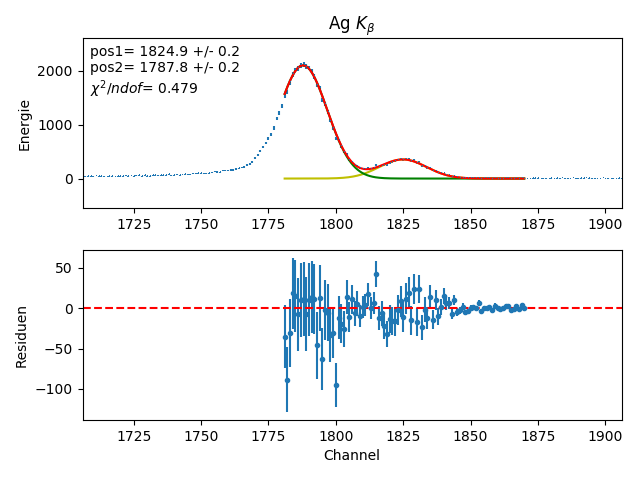
\includegraphics[scale=0.8]{Bilder/alpha/ag_beta_1.png}
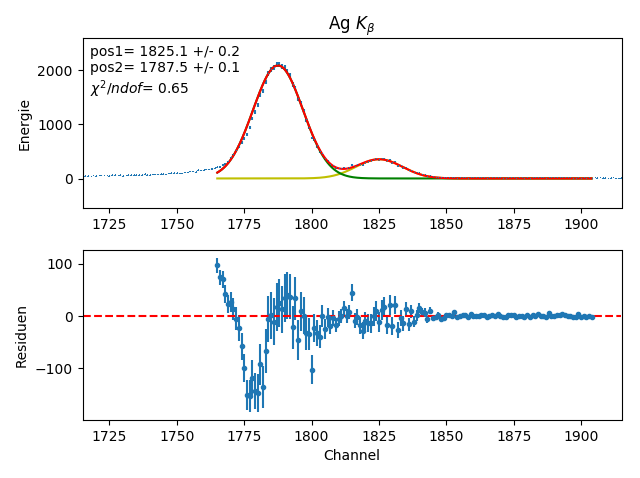
\includegraphics[scale=0.8]{Bilder/alpha/ag_beta_2.png}
\caption{Alle für dei Kalibration aufgenommenen Spektren.}
\label{fig:kal_alles}
\end{figure}

\begin{figure}[H]
\centering
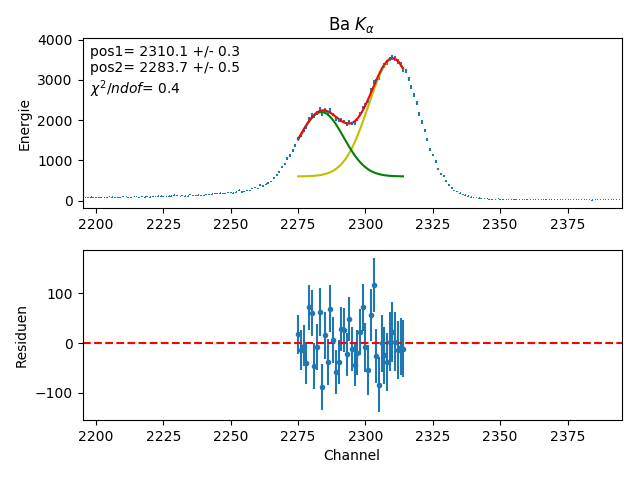
\includegraphics[scale=0.8]{Bilder/alpha/ba_alpha_1.png}
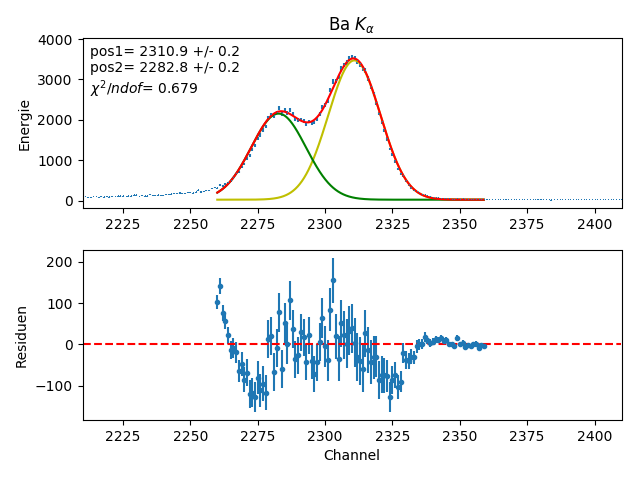
\includegraphics[scale=0.8]{Bilder/alpha/ba_alpha_2.png}
\caption{Alle für dei Kalibration aufgenommenen Spektren.}
\label{fig:kal_alles}
\end{figure}
\begin{figure}[H]
\centering
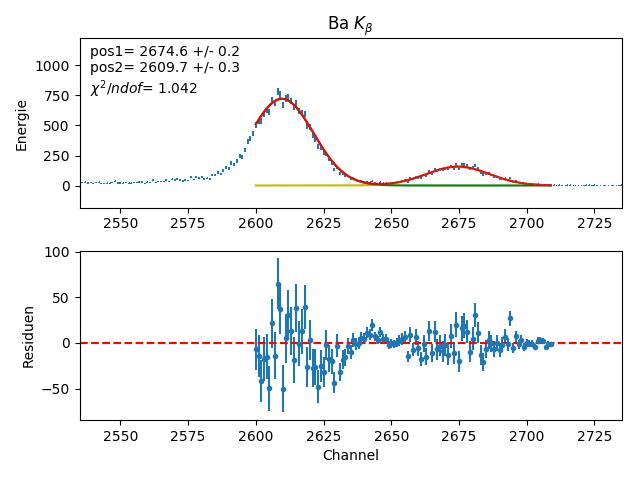
\includegraphics[scale=0.8]{Bilder/alpha/ba_beta_1.png}
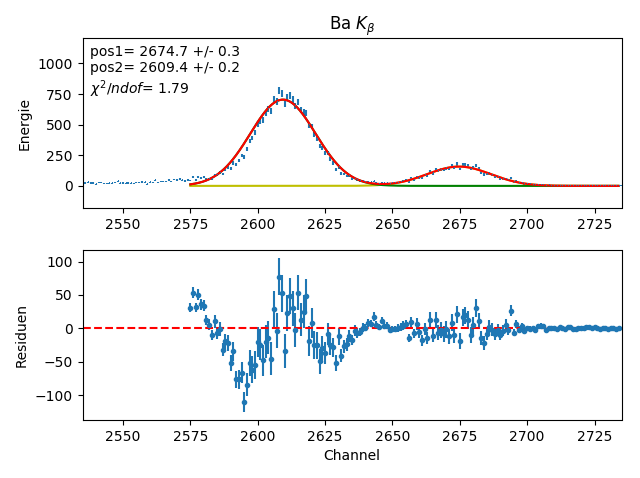
\includegraphics[scale=0.8]{Bilder/alpha/ba_beta_2.png}
\caption{Alle für dei Kalibration aufgenommenen Spektren.}
\label{fig:kal_alles}
\end{figure}

\begin{figure}[H]
\centering
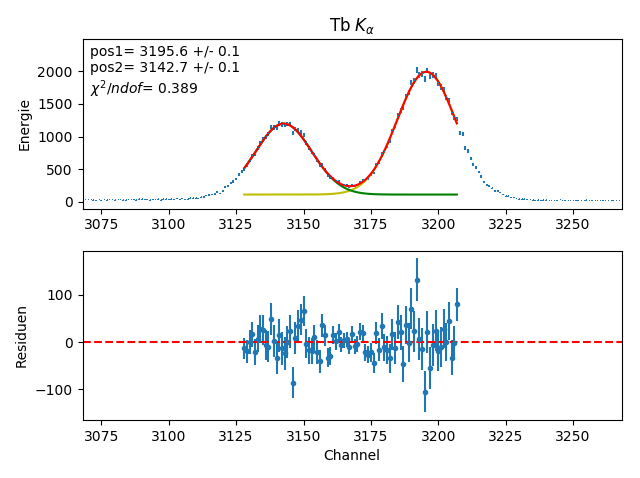
\includegraphics[scale=0.8]{Bilder/alpha/tb_alpha_1.png}
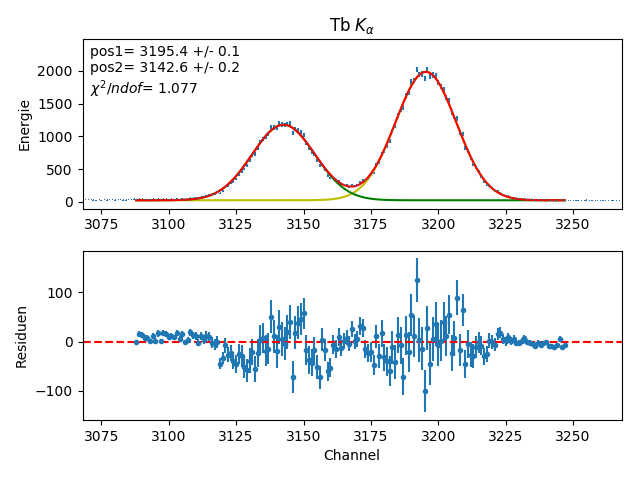
\includegraphics[scale=0.8]{Bilder/alpha/tb_alpha_2.png}
\caption{Alle für dei Kalibration aufgenommenen Spektren.}
\label{fig:kal_alles}
\end{figure}
\begin{figure}[H]
\centering
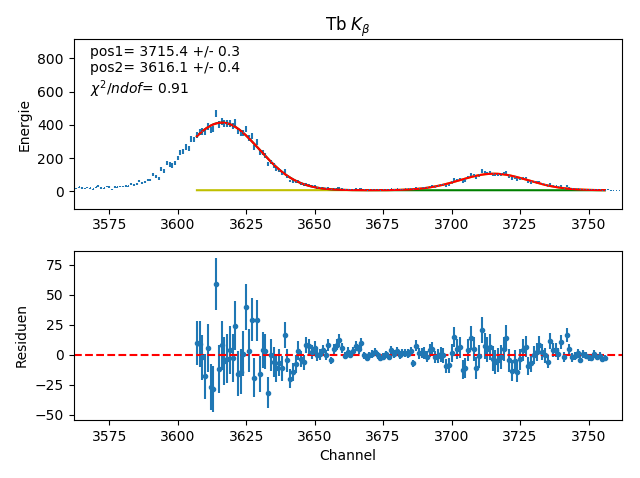
\includegraphics[scale=0.8]{Bilder/alpha/tb_beta_1.png}
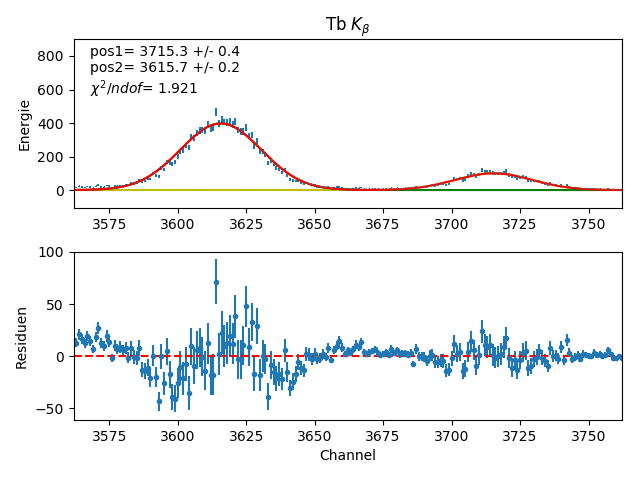
\includegraphics[scale=0.8]{Bilder/alpha/tb_beta_2.png}
\caption{Alle für dei Kalibration aufgenommenen Spektren.}
\label{fig:kal_alles}
\end{figure}

\end{document}
